\section{Attitude Model} \label{sec:AttitudeModel}
The attitude model of the quadcopter describes how the roll, pitch and yaw angles evolve according to the forces and torques exerted by the propellers. 

The free body diagrams, see \autoref{fig:droneDiagram} and \ref{fig:torquesDiagram}, are the basis for deriving the attitude model.
\vspace{-0.3 cm}
\begin{figure}[H]
  \captionbox
  {
    Free body diagram that holds both the inertial and body reference systems, as well as the references for the angles, roll, pitch and yaw, along with the thrust forces and the gravitational force.
    \label{fig:droneDiagram}
  }
  {
    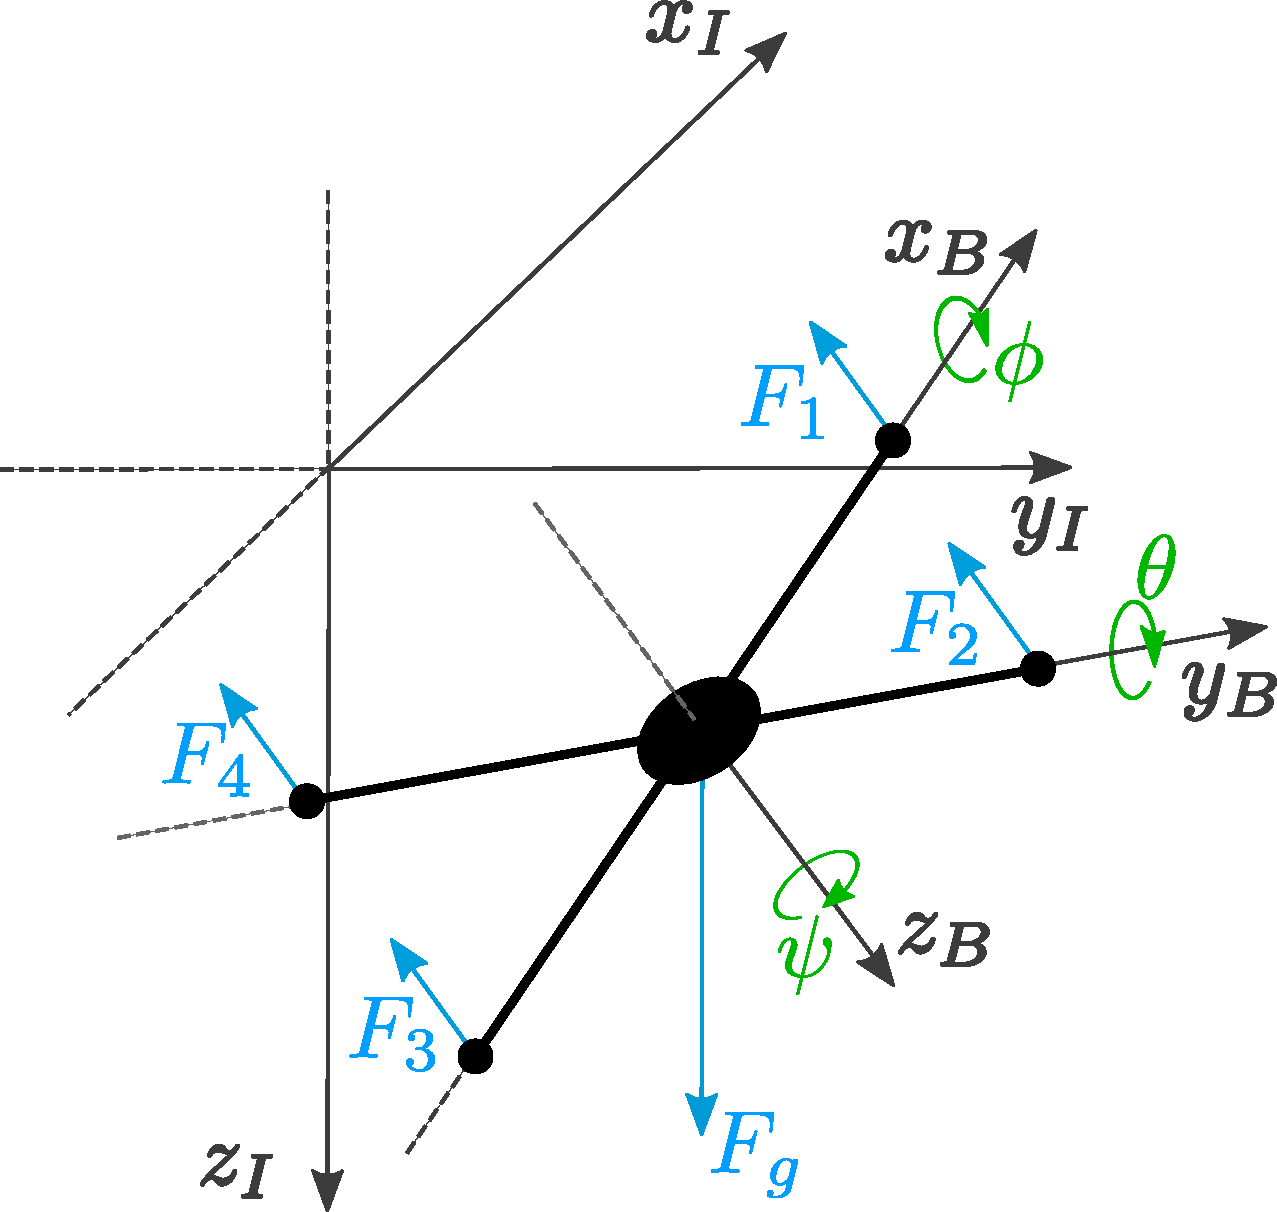
\includegraphics[width=.48\textwidth]{figures/droneDiagram}
  }
  \hspace{5pt}
  \captionbox
  {
    Free body diagram with the references for the torques produced by the drag forces at the propellers.
    \label{fig:torquesDiagram}
  }
  {
    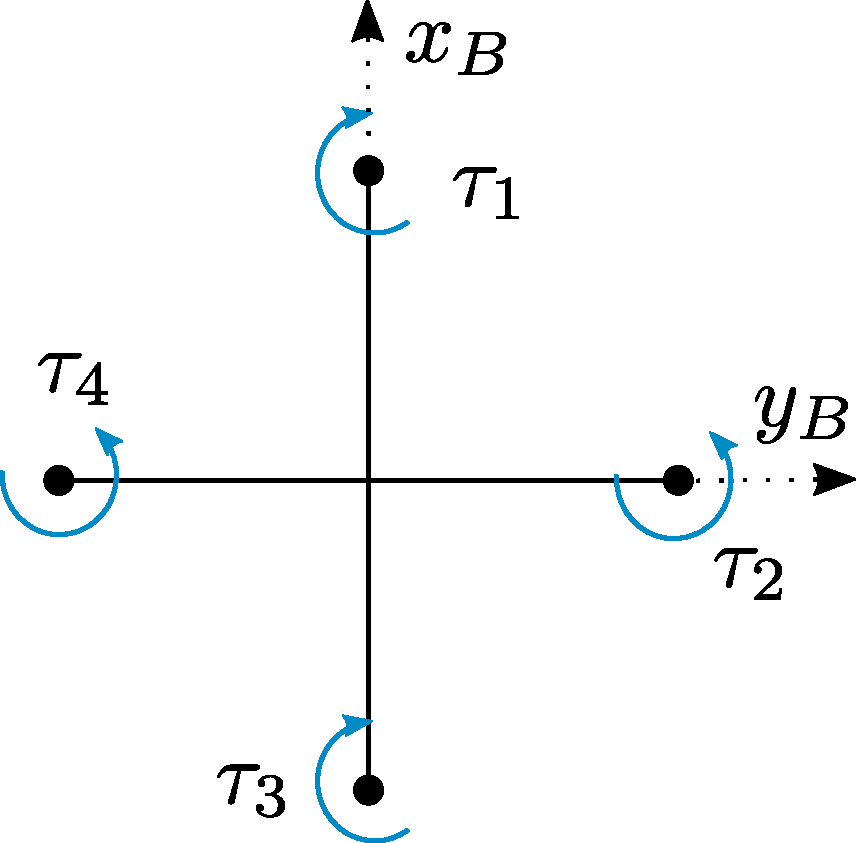
\includegraphics[width=.42\textwidth]{figures/torquesDiagram}
    \vspace{.5cm}
  }
\end{figure}
\vspace{-0.5 cm}
In \autoref{fig:droneDiagram} a free body diagram of the quadcopter is illustrated. This diagram is an extended diagram of \autoref{fig:framesDiagram} shown in \autoref{sec:ModelOverview}. Each of the thrust forces exerted by the motor and propeller is included, $F_1$, $F_2$, $F_3$ and $F_4$. Besides these four forces, the gravitational force is included as well. In \autoref{fig:torquesDiagram} the quadcopter is seen from above. Here the four torques produced by the drag forces at the propellers are illustrated. As seen in the figure, $\tau_1$ and $\tau_3$ are opposing $\tau_2$ and $\tau_4$. The motor pairs turn in opposite directions to compensate the drag torques.

From the diagrams above, the equations of angular motion around the three body axes can be derived by first principles modeling, that is, using only laws of physics. In this case, Newton's Second Law for rotational motion.
%
\begin{flalign}
	J \alpha=\sum\tau
	\label{eq:newtonangular}
\end{flalign}
\begin{where}
\va{J}{is the moment of inertia}{kg \  m^2}
\va{\alpha}{is the angular acceleration}{rad\  s^{-2}}
\va{\tau}{are the torques applied to the system}{N \  m}
\end{where}

%\begin{where}
%	\va{J}{is the moment of inertia}{kg\  m^2}
%	\va{\alpha}{is the angular acceleration}{rad\  m\  s^{-2}}
%	\va{\tau_i}{are the torques applied to the system}{Nm}
%\end{where}
%It shall be noted, that the fact that Newton's laws, that only apply in relation to an inertial reference, are applied even though the earth is accelerating and rotating, as it is the assumption, that it is of little influence for the system of the quadcopter. 
%
From applying Newton's Second Law on all three axes in the body-frame, \autoref{eq:AngleEq1}, \ref{eq:AngleEq2} and \ref{eq:AngleEq3} are obtained. As it is seen, the roll and pitch angular accelerations depend on the thrust forces exerted by the propellers placed along the $y_{\mathrm{B}}$ and $x_{\mathrm{B}}$ axes of the quadcopter, respectively. Hence the roll angular acceleration, $\ddot{\phi}$, depends on the difference in thrust force exerted by propeller four and two. Similar the pitch angular acceleration, $\ddot{\theta}$, depends on the difference in thrust force exerted by propeller one and three. The yaw angular acceleration, $\ddot{\psi}$, changes due to the torques created by the drag forces in the propellers. As the torques, $\tau_1$ and $\tau_3$, see \autoref{fig:torquesDiagram}, are pointing in the opposite direction of $\tau_2$ and $\tau_4$, the latter is subtracted from the former yielding the total torque, $J_z \ddot{\psi}$.  
\begin{align}
	J_x \ddot{\phi}&=(F_4-F_2) L  \label{eq:AngleEq1} \\
	J_y \ddot{\theta}&=(F_1-F_3) L  \label{eq:AngleEq2}\\
	J_z \ddot{\psi}&=\tau_1-\tau_2+\tau_3-\tau_4
	\label{eq:AngleEq3}
\end{align}
\begin{where}
\va{J_x}{is the inertia around $x_{\mathrm{B}}$}{kg\  m^2}
\va{J_y}{is the inertia around $y_{\mathrm{B}}$}{kg\  m^2}
\va{J_z}{is the inertia around $z_{\mathrm{B}}$}{kg\  m^2}
\va{\ddot{\phi}}{is the roll angular acceleration}{rad\  s^{-2}}
\va{\ddot{\theta}}{is the pitch angular acceleration}{rad\  s^{-2}}
\va{\ddot{\psi}}{is the yaw angular acceleration}{rad\  s^{-2}}
\va{F_i}{is the thrust force from each propeller}{N}
\va{L}{is the length from center of mass to motor}{m}
\va{\tau_i}{is the drag torque from each propeller}{N \  m}
\end{where}

%\begin{where}
%\va{\ddot{\phi}}{is roll angular acceleration}{rad $\ $ s$^{-2}$}
%\va{\ddot{\theta}}{is  pitch angular acceleration}{rad$\ $ s$^{-2}$}
%\va{\ddot{\psi}}{is yaw angular acceleration}{rad$\ $ s$^{-2}$}
%\va{J_x}{is the body moment of inertia around $x_B$ direction}{kg $\ $ m$^2$}
%\va{J_y}{is the body moment of inertia around $y_B$ direction}{kg $\ $ m$^2$}
%\va{J_z}{is the body moment of inertia around $z_B$ direction}{kg $\ $ m$^2$}
%\va{L}{is the length of the arm of the quadcopter}{m}
%\va{F_n}{is the thrust force produced in each propeller}{N}
%\va{\tau_n}{is the torque due to the drag force in each propeller}{Nm}
%\end{where}
The thrust forces and drag torques from the propeller can be assumed to be proportional to the square of the rotational speed of the motor, related by the coefficients obtained as described in \autoref{app:ThrustTest} and \ref{app:TorqueTest}. The equations above can be rewritten to include these terms.
\begin{align}
J_x \ddot{\phi}&=k_\mathrm{th} (\omega^2_4-\omega^2_2)  L \label{eq:AngleEqVelocities1}\\
J_y \ddot{\theta}&=k_\mathrm{th} (\omega^2_1-\omega^2_3)  L \label{eq:AngleEqVelocities2} \\
J_z \ddot{\psi}&=k_\mathrm{d} (\omega^2_1-\omega^2_2+\omega^2_3-\omega^2_4)
\label{eq:AngleEqVelocities3}
\end{align}
\vspace{-0.3 cm}
\begin{where}
\va{k_\mathrm{th}}{is the thrust coefficient}{N\  s^2 \  rad^{-2}}
\va{k_\mathrm{d}}{is the drag coefficient}{N \  m\  s^2 \  rad^{-2}}
\end{where}
%

\autoref{eq:AngleEqVelocities1}, \ref{eq:AngleEqVelocities2} 
and \ref{eq:AngleEqVelocities3} are the final attitude model expressions. %Now that the attitude model is known, the translational model must be derived. This is done in the following section. 